\section{Kinematic Inversion}

This section are described all the kinematic inversion procedures used to compute joint angles for the Aarm.

While direct kinematics equations provides a unique representation of the end-effector pose once joint variables are known, the problem of finding the joint variables given an end-effector pose,i.e inverse kinematics , is not any more straightforward. This is due to several reasons like the existence of multiple or infinite solutions for instance in cases of redundant manipulator.

\subsection{Linear Kinematics Inversion}
\label{ssec:lik}
In this stage the kinematic inversion problem is faced exploiting the geometric properties of the Aarm, in particular, due to the existence of multiple solutions for a given end-effector pose, will be necessary to impose some constraint on the configuration to be adopted for the manipulator.

Analysing the geometry of the manipulator it's possible to note that the kinematic inversion can be decoupled in two different sub-problems, one relative to the position and one to the orientation. In fact compute the kinematic inversion relative to arm's shoulder and elbow (joint 1,2 and 3) it is independent to the same problem relative to arm's spherical wrist (joint 4,5 and 6). A simple procedure to prove this is the following:
\begin{itemize}
	\item Given a certain end-effector position $p_e$, it is possible to compute the centre of the spherical wrist as: $p_W = p_e - d_6\hat{z_e}$
	\item Compute $\left(q_1,q_2,q_3\right)$ solving the first sub-problem, i.e kinematics inversion for the arm without wrist.
	\item Compute $R^0_3(q_1,q_2,q_3)$
	\item Compute $R^3_6(q_4,q_5,q_6) = R^{0T}_3R$, with $R$ rotation matrix extracted from the homogeneous transformation relative to pose $p_e$.
	\item Compute $\left(q_4,q_5,q_6\right)$ solving the second sub-problem, i.e kinematics inversion for the spherical wrist.
\end{itemize}

Let's now analyse the two sub-kinematic inversion separately beginning from the shoulder-elbow part.

\subsubsection{Shoulder-Elbow angles}
\label{ssec:seangle}
The wrist position is computed as follows:

\begin{center}
	$\begin{cases}
		p_{Wx}=\cos{(q_1)}\left(a_2\cos{(q_2)}+d_4\cos{(q_1+q_3)}\right)\\
		p_{Wy}=\sin{(q_1)}\left(a_2\cos{(q_2)}+d_4\cos{(q_1+q_3)}\right)\\
 		p_{Wy}=a_2\sin{(q_2)}+a_2\sin{(q_2+q_3)}
	\end{cases}$
\end{center}

After squaring and summing above equations it's possible to solve the resulting one for $\cos(q_3)$ whose expression is not reported for sake of briefness. Then imposing $-1<\cos(q_3)<1$ we can obtain also 
\begin{center}
	$\sin(q_3) = \pm\sqrt{1 - \cos(q_3)^2}$
\end{center}
Through $\sin(q_3)$ and $\cos(q_3)$ is possible to find
\begin{center}
	 $q_{3_{1,2}} = \arctan2(\pm\sin{(q_3)},\cos{(q_3)})$
\end{center}
By means $q_3$, after squaring ad summing firs two equations of $p_W$ it's possible to compute $\sin(q_2)$ and $\cos(q_2)$, each can assuming two different values. Moving straightforward to the solution it's possible to prove that $q_2$ can assume four different values $q_{2,1}, q_{2,2}, q_{2,3}, q_{2,4}$ corresponding to the sings chosen for $q_3$ in both resulting formulas.\newline
Finally $q_1$ can be computed from first 2 equations of $p_W$ as function of $q_2$ and $q_3$
\begin{center}
	$q_{1_{1,2}} = \arctan2(\pm p_{Wy},\pm p_{Wx}) $
\end{center}
As result the combination of above three angles lead to the specification of four possible configuration for the manipulator, Fig.\ref*{fig:aarmeud} shows two of those namely \textit{Elbow-Up}, $\left(q_{1_{1,2}},q_{2_3},q_{3_2}\right)$, and \textit{Elbow-Down} $(q_{1_{1,2}},q_{2_1},q_{3_1})$.

\begin{figure}[h]
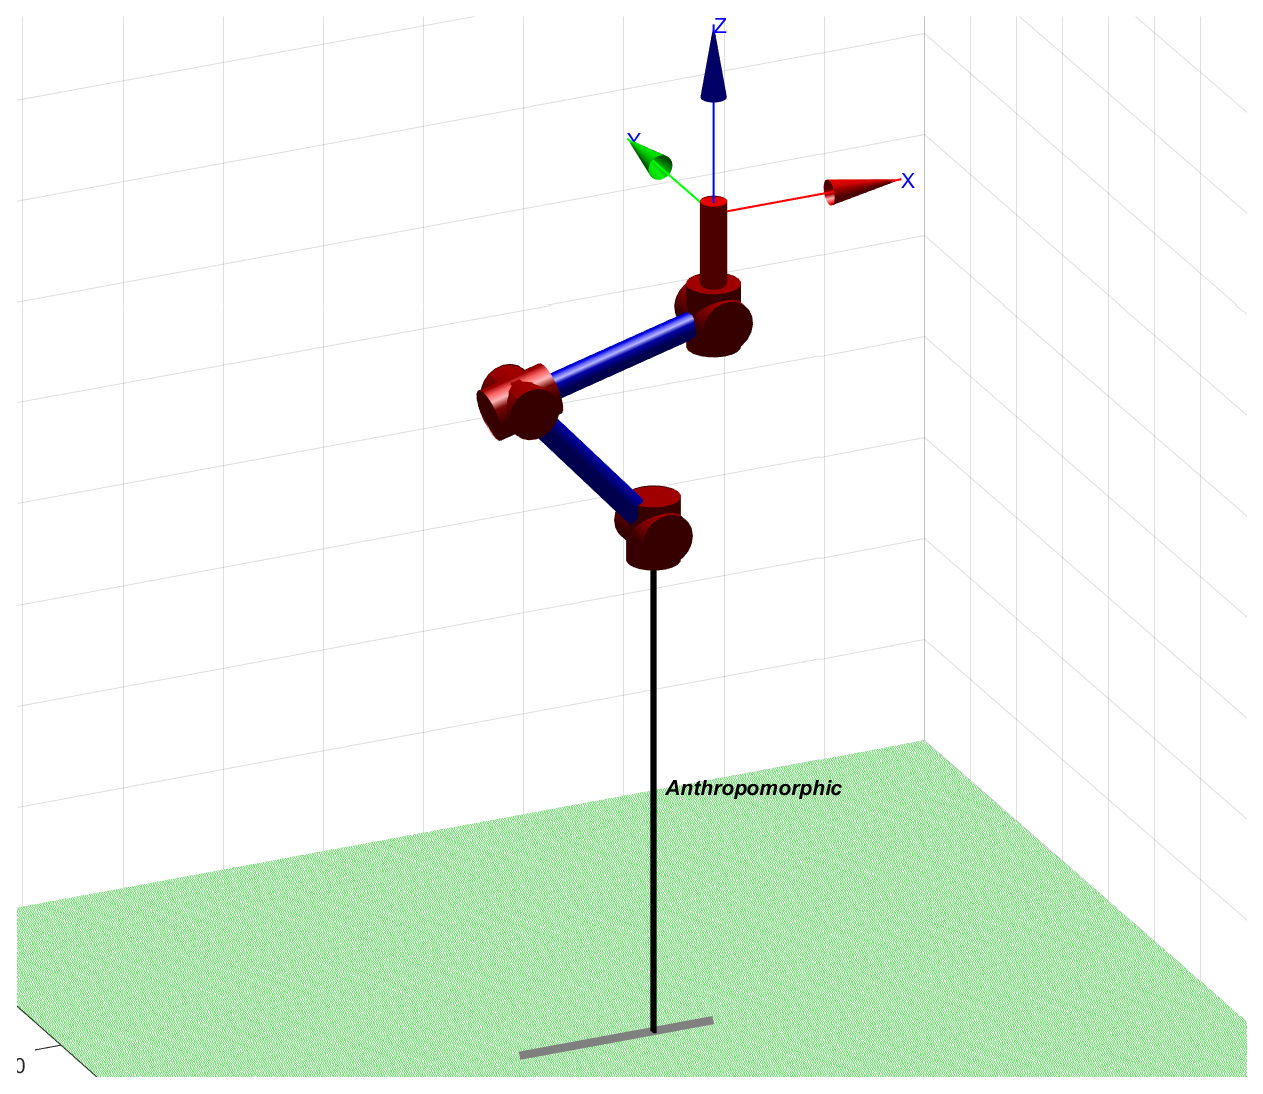
\includegraphics[width=0.5\linewidth]{img/aarmeu}\quad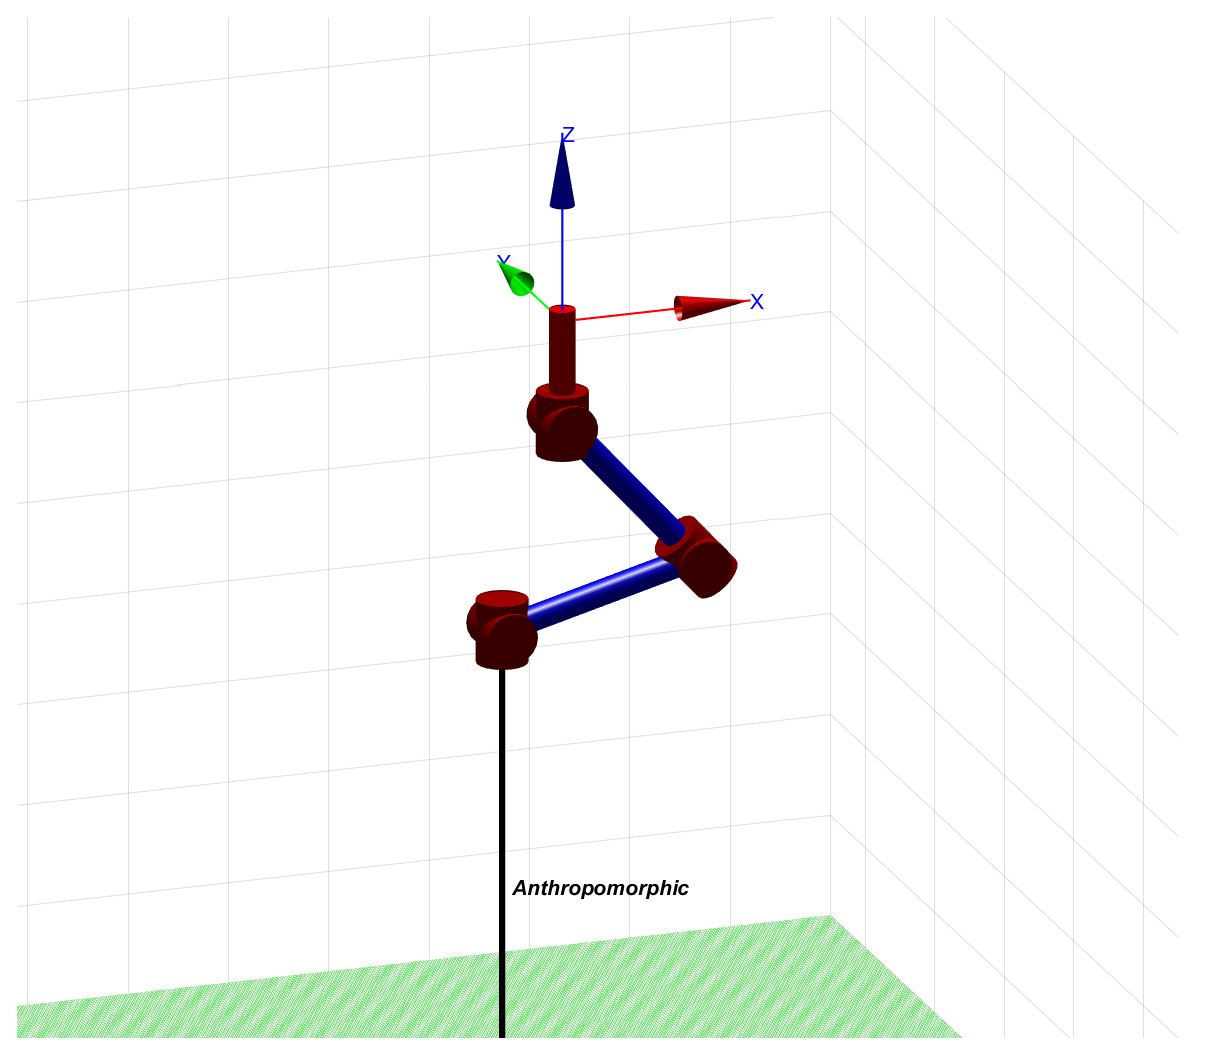
\includegraphics[width=0.5\linewidth]{img/aarmed}
\caption{Elbow-Up and Elbow-Down Configurations}
\label{fig:aarmeud}
\end{figure}
The other two possible configuration are same as above with angle $q_1$ rotated by $\pi$ so the difference is not clearly visible.

\subsubsection{Wrist angles}
\label{ssec:wangles}
Spherical-Wrist joint angles can be computed from the intermediate rotation matrix 
\begin{center}
	$R^3_6 = \left(
	\begin{matrix}
		n^3_x & s^3_x & a^3_x \\
		n^3_y & s^3_y & a^3_y \\
		n^3_z & s^3_z & a^3_z		
	\end{matrix}
	\right)$	
\end{center}
Which represents the Euler angles with respect to frame 3. Even in this cases joint angles can assume different values based on the equations solving, in particular
\begin{center}
$q_{4_{1,2}} = \arctan2(\pm a^3_y, \pm a^3_x)$
\end{center}
\begin{center}
$q_{5_{1,2}} = \arctan2(\pm\sqrt{(a^3_y)^2+(a^3_x)^2}, a^3_z) $
\end{center}
\begin{center}
	$q_{6_{1,2}} = \arctan2(\pm s^3_z, \mp n^3_z)$
\end{center}

From above joint angles it is possible to determine two different wrist configurations, one having $q_5 \in \left(0, \pi\right)$, i.e $(q_{1_1},q_{2_1},q_{3_1}) $, and the other having  $q_5 \in \left(-\pi, 0\right)$, i.e $(q_{1_2},q_{2_2},q_{3_2})$.

\subsubsection{Implementation}

The implementation of the linear kinematics inversion described above starts from the choice on what configuration impose to the robotic arm during the task execution, being the shape to be cut in the horizontal plane the \textit{Elbow-Up} plus \textit{Shoulder-Front} configuration was preferred, while for what concern the wrist no specific advantages are due to the choice of one configuration in place of the other.

The function that performs the kinematic inversion is the following
\begin{lstlisting}
function q = ikineAarmSW(robot, T)
pe = T2Coords(T);
pw = pe(1:3) + [0 0 robot.d(6)];
q(1:3) = ikineAarm(pw, [0 robot.a(2) robot.d(4)], 'sbeu');
q(3) = q(3) + pi/2;
R = t2r(T);
R03 = t2r(SerialLink(robot.links(1:3)).fkine(q(1:3)));
R36 = R03'*R;
q(4:6) = ikineSW(R36, '-pi0');
end
\end{lstlisting}
where function
\begin{lstlisting}
pe = T2Coords(T);
\end{lstlisting}
simply extracts position coordinates from an homogeneous matrix and function  
\begin{lstlisting}
q = ikineAarm(pw, [0 robot.a(2) robot.d(4)], 'sbeu');
\end{lstlisting}
exploits the computations explained in \ref{ssec:seangle} to retrieve first three joint angles taking as input the wrist position, links dimension and manipulator configuration. The second sub-kinematics inversion for a specific wrist configuration is performed through function
\begin{lstlisting}
q = ikineSW(R36, '-pi0');
\end{lstlisting}
by means of \ref{ssec:wangles} formulas.
\newpage
\subsection{Differential Kinematics Inversion}
\label{ss:dki}
Another technique used to solve the inverse kinematics could be used in cases in which the above solution it's difficult to perform, e.g no easy closed-form could be found, or one wants to exploit some manipulator features in order to optimize secondary objective functions. Such technique comes directly from the \textit{Fundamental Differential Kinematics} formula
\begin{center}
	$v_e  = J(q)\dot{q}$
\end{center}
which ties end-effector and joint velocities by means the so called Jacobian matrix. Hence joint velocity could be obtained simply inverting the above relation
\begin{center}
	$\dot{q} = J^{-1}(q)v_e$
\end{center}
A first problem is to determine whether the Jacobian matrix is invertible, a necessary condition is that it's a square matrix. When a robot is intrinsically redundant it never happens, since $J$ has at most 6 rows and $n$ columns, with $n>6$ number of joints. On the other side if the robot is not intrinsically redundant, i.e $n\leqslant6$, but redundant with respect to an assigned task, i.e $n > r$ with $r$ number of DOF required from that task, the $J$ matrix could be square but one, or more, of its rows is useless. That's exactly the case of the laser-cutting anthropomorphic arm, it is sufficient to note that in order to perform the task the information provided by the $6^{th}$ coordinate of the end-effector velocity $v_e$, i.e $\omega_z$ , is not needed any more. Hence it is possible to remove the $6^{th}$ row of $J$ thus making it a $5\times6$ matrix.

Now $J$ is not square any more, so there exist more than one solution of the differential kinematics formula; a common way to face with this kind of problem is to find solutions $\dot{q}$ that minimize the quadratic cost functional of joint velocities
\begin{center}
	$g(\dot{q})=\dfrac{1}{2}\dot{q}^TW\dot{q}$
\end{center}
where $W$ is a weight matrix, positive definite. Hence the solution of the problem
\begin{center}
	$\begin{cases}
		min\left(g(\dot{q})\right) \\
		v_e = J(q)\dot{q}
	\end{cases}$
\end{center}
becomes
\begin{center}
$	\dot{q} = W^{-1}J^T(JW^{-1}J^T)v_e$
\end{center}
and in the case in which $W = I$
\begin{center}
$	\dot{q} = J^T(JJ^T)v_e$
\end{center}
and said $J^\dagger=J^T(JJ^T)^{-1}$ \textit{right pseudo-inverse of Jacobian}, the final result is
\begin{center}
	$\dot{q} = J^\dagger(q)v_e$
\end{center}
Which allow to compute joint velocities from end-effector velocities. Once obtained $\dot{q}$ it is possible to perform a numerical integration to retrieve $q$ as follow
\begin{center}
	$q(t_{i+1})=q(t_i) + \dot{q}(t_i)dt$
\end{center}
with $dt$ time interval between two consecutive points of the trajectory.
\newpage
\subsubsection{Open-Loop Implementation}
\label{sssec:olimp}
The above procedure has been implemented in Matlab using also some utilities of the \textit{Robotics Toolbox}.
The main function is
\begin{lstlisting}
function [q, qend, man] = iDiffKine(robot, Ttg, dt, q)
\end{lstlisting}
Which taking as input \textit{robot}, \textit{Ttg} that is the set of homogeneous matrix corresponding to each point of the trajectory, \textit{dt} and an initial joint pose $q0$, returns the set of joint angles $q$ for each point and the final angle $q_e$. At every step the function estimate the end-effector velocity through a numeric derivation
\begin{center}
$	v_{e,i} = \dfrac{p_i - p_{i-1}}{dt}$
\end{center}
Follows the whole implementation of the \textit{iDiffKine} function
\begin{lstlisting}
function [q, qend] = iDiffKine(robot, Ttg, dt, q, opt)
   steps = size(Ttg,3);
   qcurr = q;
   Tprev = Ttg(:,:,1);
   for i=1:steps
       Tcurr = Ttg(:,:,i);
       prev = T2Coords(Tprev);
       new = T2Coords(Tcurr);
       dVe = (new - prev)/dt;
       dVe = dVe(1:5);
       J = robot.jacob0(qcurr);
       J = J(1:5,:);
       Jpi = J'*((J*J')^-1);
       dqcurr = (Jpi*dVe')'; 
       qcurr = qcurr + dqcurr*dt;
       q(:,i) = qcurr;
       Tprev = Tcurr;
   end
   qend = qcurr;
end   
\end{lstlisting}
The function \textit{jacob0(q)} is provided by the \textit{Robotics Toolbox} and given a joint angles $q$ returns the Jacobian matrix with respect to frame 0.

\subsubsection{Improvements}
\label{sssec:ikcon}

The implementation provided in \ref{sssec:olimp} provide solutions according to an open-loop scheme, at every step a new $q$ is computed, but of course, due to the numerical integration, it could drift from the desired one. A possible solution to mitigate such phenomenon is taking into account the error made at every step and then try to minimize it, there is a built-in function in \textit{Robotics Toolbox} that exactly performs what said
\begin{lstlisting}
    q = robot.ikcon(T);
\end{lstlisting}
Taking as input the homogeneous transformation relative to the end-effector pose.% and return joint angles that solves the following optimization problem:
%\begin{center}
%$\begin{cases}
%min\quad sumsqr\left( T^{-1}T^b_e(q) - I\omega \right) \\
%q \leqslant qub \\
%q \leqslant -qlb
%\end{cases}$
%\end{center}
%Where the objective function express the error $e$ in the pose $T$ with $\omega$ weight matrix not modifiable. The additional constraints express the condition of $q$ inside the joint limits.
\newpage
\subsection{Null-Space optimization}

As far the arm redundancy with respect to the assigned task had the only effect to change the way to compute the inverse matrix that multiplies end-effector velocity in order to get joint velocities, the kinematic redundancy explication make sense when becomes possible exploit it to optimize secondary objective functions. Being $n-r$ the dimension of Jacobian \textit{null space}, if $\tilde{\dot{q}}$ solves $v_e = J(q)\dot{q}$ then also
\begin{center}
	$\dot{q} = \tilde{\dot{q}} + P\dot{q_0}$
\end{center}
solves it, being $P$ a matrix which project an arbitrary joint velocity vector $\dot{q_0}$ in the null space ($P\dot{q_0}=0$)
\begin{center}
	$J\dot{q} = J\tilde{\dot{q}} + JP\dot{q_0} = v_e$
\end{center}
Now problem of \ref{ss:dki} can be rewritten, using the additional vector $q_0$, as
\begin{center}
	$\begin{cases}
	\min \dfrac{1}{2}(\dot{q} - \tilde{\dot{q_0}})^T(\dot{q} - \tilde{\dot{q_0}})\\
	v_e = J(q)\dot{q}
	\end{cases}$
\end{center}
Which means to find those solutions subjected to the constraint $v_e = J(q)\dot{q}$ which minimizes the norm of vector $(\dot{q} - \tilde{\dot{q_0}})$ and hence are as close as possible to vector $\tilde{\dot{q_0}}$. In this way the additional objective functions can be specified by means $\tilde{\dot{q_0}}$. Solving the above problem leads to 
\begin{center}
	$\dot{q} = J^\dagger v_e + (I-J^\dagger J)\tilde{\dot{q_0}}$
\end{center}
where $(I-J^\dagger J)$ is a possible $P$ matrix. Now let 
\begin{center}
	$\dot{q_0} = k_0\left(\dfrac{\partial w(q)}{\partial q}\right)$
\end{center}
$w(q)$ corresponds the secondary objective function, that in this work has been set to a typical measure namely \textit{manipulability}. Such measure is usually adopted as distance of manipulator from singular configurations. 
\begin{center}
$w(q) = \sqrt{det(J(q)J(q)^T)}$
\end{center}

\subsubsection{Implementation}

First problem to face with is that by means the \textit{Robotic Toolbox} functions is possible to obtain numeric evaluation of the manipulator quantities, but not their analytical expressions, thus creating the need to compute the gradient of $w(q)$ numerically. Let's try to explain such concept by considering the \textit{manipulability} expression $\sqrt{det(J(q)J(q)^T)}$, in order to compute its gradient it is necessary to express it in an analytical form, but as long $J$ is calculated through the \textit{Robotics Toolbox} function \textit{robot.jacob0(q)} only a numerical evaluation is provided. A possible way is to derive the analytical expression of $J$ and then obtain the corresponding analytical expression of $w(q)$ thus allowing also the computation of its gradient expression, this is in practice very difficult since even for simple manipulator the analytical expression can be very complicated. Another possibility is to directly compute it with a numerical procedure. Referring to this second case the way adopted in this work is to use the \textit{Matlab Optimzation Toolbox}. The problem is to find a value $\dot{q^*_0}$ which maximizes the function $w(q)$ could be formulated as an unconstrained optimization problem to be solved by means \textit{fminunc} function
\begin{lstlisting}
optFunction = @(x) manipulabilityOF(x, robot, k0, dt);
opt = optimoptions('fminunc','Algorithm','quasi-newton','Display','off');	
[dq0] = fminunc(optFunction, dq0, opt);
\end{lstlisting}
The objective functions is defined as follow
\begin{lstlisting}
function m = manipulabilityOF(dq0, robot, k0, dt)
J = robot.jacob0(q);
J = J(1:5,:);
nj = size(robot.qlim, 1);
I = eye(nj);
J_pinv = J'*((J*J')^-1);
dq0 = J_pinv*dVe' + (I-J_pinv*J)*dq0'*k0;
q = q + dq0'*dt;
J = robot.jacob0(q);
J = J(1:5,:);
m = -sqrt(det(J*J'));
end
\end{lstlisting}

Once the value of $\dot{q_0}$ has been determined the new joint angle can be simply computed as
\begin{lstlisting}
[dq0] = fminunc(optFunction, dq0, opt);
dqcurr = dqcurr + (I-Jpi*J)*dq0'*k0;
q = qcurr + dqcurr'*dt;
\end{lstlisting}

It's important to notice how such procedure slows down the performance of the algorithm due to computational heaviness, a deeper discussion on this will be make in \ref{sec:rpe}. Another things to take into account is the value of constant $k_0$, which represents the optimization contribute to the displacement, it should be tuned in base on the iterations number $n$, in particular for high values of it $k_0$ should be smaller to spread its contribute among more iterations and vice-versa.